% !TeX spellcheck = sl_SI
% vim: set spell spelllang=sl:
% za preverjanje črkovanja, če se uporablja Texstudio ali vim
\documentclass[12pt,a4paper,twoside]{article}
\usepackage[utf8]{inputenc}  % pravilno razpoznavanje unicode znakov

% NASLEDNJE UKAZE USTREZNO POPRAVI
\newcommand{\program}{Pedagoška matematika} % ime studijskega programa
\newcommand{\imeavtorja}{Simon Besednjak} % ime avtorja
\newcommand{\imementorja}{prof.~dr.~Marjetka Knez} % akademski naziv in ime mentorja, uporabi poln naziv, prof.~dr.~, doc.~dr., ali izr.~prof.~dr.
\newcommand{\imesomentorja}{} % akademski naziv in ime somentorja, če ga imate
\newcommand{\naslovdela}{Dvojne PH krivulje}
\newcommand{\letnica}{2021} % letnica magistriranja
\newcommand{\opis}{Delo obravnava lastnosti krivulj z pitagorejskih hodografom.}  % Opis dela v eni povedi. Ne sme vsebovati matematičnih simbolov v $ $.
\newcommand{\kljucnebesede}{PH krivulje\sep dvojne PH krivulje} % ključne besede, ločene z \sep, da se PDF metapodatki prav procesirajo
\newcommand{\keywords}{PH curves\sep double PH curves} % ključne besede v angleščini
\newcommand{\organization}{Univerza v Ljubljani, Fakulteta za matematiko in fiziko} % fakulteta
\newcommand{\literatura}{literatura}  % pot do datoteke z literaturo (brez .bib končnice)
\newcommand{\sep}{, }  % separator med ključnimi besedami v besedilu
% KONEC PODATKOV

\usepackage{bibentry}         % za navajanje literature v programu dela s celim imenom
\nobibliography{\literatura}
\newcommand{\plancite}[1]{\item[\cite{#1}] \bibentry{#1}} % citiranje v programu dela

\usepackage{filecontents}  % za pisanje datoteke s PDF metapodatki
\usepackage{silence} \WarningFilter{latex}{Overwriting file}  % odstrani annoying warning o obstoju datoteke
% datoteka s PDF metapodatki, zgenerira se kot magisterij.xmpdata
\begin{filecontents*}{\jobname.xmpdata}
  \Title{\naslovdela}
  \Author{\imeavtorja}
  \Keywords{\kljucnebesede}
  \Subject{matematika}
  \Org{\organization}
\end{filecontents*}

\usepackage[a-1b]{pdfx}  % zgenerira PDF v tem PDF/A-1b formatu, kot zahteva knjižnica
\hypersetup{bookmarksopen, bookmarksdepth=3, colorlinks=true,
  linkcolor=black, anchorcolor=black, citecolor=black, filecolor=black,
  menucolor=black, runcolor=black, urlcolor=black, pdfencoding=auto,
  breaklinks=true, psdextra}

\usepackage[slovene]{babel}  % slovenščina
\usepackage[T1]{fontenc}     % naprednejše kodiranje fonta
\usepackage{amsmath,amssymb,amsfonts,amsthm} % matematični paketi
\usepackage{graphicx}     % za slike
\usepackage{emptypage}    % prazne strani so neoštevilčene, ampak so štete
\usepackage{units}        % fizikalne enote kot \unit[12]{kg} s polovico nedeljivega presledka, glej primer v kodi
\usepackage{makeidx}      % za stvarno kazalo, lahko zakomentiraš, če ne rabiš
\makeindex                % za stvarno kazalo, lahko zakomentiraš, če ne rabiš
% oblika strani
\usepackage[
  top=3cm,
  bottom=3cm,
  inner=3.5cm,      % margini za dvostransko tiskanje
  outer=2.5cm,
  footskip=40pt     % pozicija številke strani
]{geometry}

% VEČ ZANIMIVIH PAKETOV
% \usepackage{array}      % več možnosti za tabele
% \usepackage[list=true,listformat=simple]{subcaption}  % več kot ena slika na figure, omogoči slika 1a, slika 1b
% \usepackage[all]{xy}    % diagrami
% \usepackage{doi}        % za clickable DOI entrye v bibliografiji
% \usepackage{enumerate}     % več možnosti za sezname

% Za barvanje source kode
% \usepackage{minted}
% \renewcommand\listingscaption{Program}

% Za pisanje psevdokode
% \usepackage{algpseudocode}  % za psevdokodo
% \usepackage{algorithm}
% \floatname{algorithm}{Algoritem}
% \renewcommand{\listalgorithmname}{Kazalo algoritmov}

% DRUGI TVOJI PAKETI:
% tukaj
\newcommand{\iu}{\mathrm{i}\mkern1mu} % za imaginarno enoto
%\allowdisplaybreaks

\setlength{\overfullrule}{50pt} % označi predlogo vrstico
\pagestyle{plain}               % samo številka strani na dnu, nobene glave / noge

% ukazi za matematična okolja
\theoremstyle{definition} % tekst napisan pokončno
\newtheorem{definicija}{Definicija}[section]
\newtheorem{primer}[definicija]{Primer}
\newtheorem{opomba}[definicija]{Opomba}
\newtheorem{aksiom}{Aksiom}

\theoremstyle{plain} % tekst napisan poševno
\newtheorem{lema}[definicija]{Lema}
\newtheorem{izrek}[definicija]{Izrek}
\newtheorem{trditev}[definicija]{Trditev}
\newtheorem{posledica}[definicija]{Posledica}

\numberwithin{equation}{section}  % števec za enačbe zgleda kot (2.7) in se resetira v vsakem poglavju

% Matematični ukazi
\newcommand{\R}{\mathbb R}
\newcommand{\N}{\mathbb N}
\newcommand{\Z}{\mathbb Z}
\renewcommand{\C}{\mathbb C}
\newcommand{\Q}{\mathbb Q}
\newcommand{\tangenta}{\frac{\mathbf{r}'}{\lVert \mathbf{r}'\rVert}}
\newcommand{\normala}{\frac{\mathbf{r}'\times\mathbf{r}''}{\lVert \mathbf{r}'\times\mathbf{r}'' \rVert}\times \mathbf{t}}
\newcommand{\binormala}{\frac{\mathbf{r}'\times\mathbf{r}''}{\lVert \mathbf{r}'\times\mathbf{r}'' \rVert}}
\newcommand{\fleksija}{\frac{\lVert \mathbf{r}'\times\mathbf{r}'' \rVert}{\sigma^3}}
\newcommand{\torzija}{\frac{(\mathbf{r}'\times\mathbf{r}'')\cdot\mathbf{r}'''}{\lVert \mathbf{r}'\times\mathbf{r}'' \rVert^2}}
\newcommand{\tV}{\mathbf{t}}
\newcommand{\aV}{\mathbf{a}}
\newcommand{\bV}{\mathbf{b}}
\newcommand{\pV}{\mathbf{p}}
\newcommand{\rV}{\mathbf{r}}
\newcommand{\iV}{\mathbf{i}}
\newcommand{\jV}{\mathbf{j}}
\newcommand{\kV}{\mathbf{k}}
\newcommand{\ndr}{\lVert \mathbf{r}'\rVert} % norma prvega odvoda
\newcommand{\ndrtddr}{\lVert \mathbf{r}'\times \mathbf{r}'' \rVert} % norma vektorskega produkta prvega in drugega odvoda
\newcommand{\AQ}{\mathcal{A}}
\newcommand{\BQ}{\mathcal{B}}
\newcommand{\CQ}{\mathcal{C}}
\newcommand{\boldalpha}{\boldsymbol \alpha}
\newcommand{\boldbeta}{\boldsymbol \beta}

% \DeclareMathOperator{\tr}{tr}  % morda potrebuješ operator za sled ali kaj drugega?

% bold matematika znotraj \textbf{ }, tudi v naslovih, kot \omega spodaj
\makeatletter \g@addto@macro\bfseries{\boldmath} \makeatother

% Poimenuj kazalo slik kot ``Kazalo slik'' in ne ``Slike''
\addto\captionsslovene{
  \renewcommand{\listfigurename}{Kazalo slik}%
}

% če želiš, da se poglavja začnejo na lihih straneh zgoraj
% \let\oldsection\section
% \def\section{\cleardoublepage\oldsection}

%%%%%%%%%%%%%%%%%%%%%%%%%%%%%%%%%%%%%%%%%%
%%%%%%           DOCUMENT           %%%%%%
%%%%%%%%%%%%%%%%%%%%%%%%%%%%%%%%%%%%%%%%%%

\begin{document}

\pagenumbering{roman} % začnemo z rimskimi številkami
\thispagestyle{empty} % ampak na prvi strani ni številke

\noindent{\large
UNIVERZA V LJUBLJANI\\[1mm]
FAKULTETA ZA MATEMATIKO IN FIZIKO\\[5mm]
\program\ -- 2.~stopnja}
% ustrezno dopolni za IŠRM
\vfill

\begin{center}
  \large
  \imeavtorja\\[3mm]
  \Large
  \textbf{\MakeUppercase{\naslovdela}}\\[10mm]
  \large
  Magistrsko delo \\[1cm]
  Mentor: \imementorja \\[2mm] % ustrezno popravi spol
%   Somentor: \imesomentorja   % dodaj, če potrebno
\end{center}
\vfill

\noindent{\large Ljubljana, \letnica}

\cleardoublepage

%% sem pride IZJAVA O AVTORSTVU  -- SE NATISNE V VIS

% zahvala
\pdfbookmark[1]{Zahvala}{zahvala} %
\section*{Zahvala}
Neobvezno.
Zahvaljujem se \dots
% end zahvala -- izbriši vse med zahvala in end zahvala, če je ne rabiš

\cleardoublepage

\pdfbookmark[1]{\contentsname}{kazalo-vsebine}
\tableofcontents

% list of figures
% \cleardoublepage
% \pdfbookmark[1]{\listfigurename}{kazalo-slik}
% \listoffigures
% end list of figures

\cleardoublepage

\section*{Program dela}
\addcontentsline{toc}{section}{Program dela} % dodajmo v kazalo
Mentor naj napiše program dela skupaj z osnovno literaturo. Na literaturo se
lahko sklicuje kot~\cite{lebedev2009introduction}, \cite{gurtin1982introduction},
\cite{zienkiewicz2000finite}, \cite{STtemplate}.

\section*{Osnovna literatura}
Literatura mora biti tukaj posebej samostojno navedena (po pomembnosti) in ne
le citirana. V tem razdelku literature ne oštevilčimo po svoje, ampak uporabljamo
okolje itemize in ukaz plancite, saj je celotna literatura oštevilčena na koncu.
\begin{itemize}
  \plancite{DPHclanek1}
  \plancite{DPHclanek2}
  \plancite{farouki2008pythagorean}
\end{itemize}

\vspace{2cm}
\hspace*{\fill} Podpis mentorja: \phantom{prostor za podpis}

% \vspace{2cm}
% \hspace*{\fill} Podpis somentorja: \phantom{prostor za podpis}

\cleardoublepage
\pdfbookmark[1]{Povzetek}{abstract}

\begin{center}
\textbf{\naslovdela} \\[3mm]
\textsc{Povzetek} \\[2mm]
\end{center}
Tukaj napišemo povzetek vsebine. Sem sodi razlaga vsebine in ne opis tega, kako je delo
organizirano.

\vfill
\begin{center}
\textbf{English translation of the title} \\[3mm] % prevod slovenskega naslova dela
\textsc{Abstract}\\[2mm]
\end{center}

An abstract of the work is written here. This includes a short description of
the content and not the structure of your work.

\vfill\noindent
\textbf{Math.~Subj.~Class.~(2010):} oznake kot 74B05, 65N99, na voljo so na naslovu
\url{http://www.ams.org/msc/msc2010.html} \\[1mm]
\textbf{Ključne besede:} \kljucnebesede \\[1mm]
\textbf{Keywords:} \keywords

\cleardoublepage

\setcounter{page}{1}    % od sedaj naprej začni zopet z 1
\pagenumbering{arabic}  % in z arabskimi številkami

%%%%%%%%%%%%%%%%%%%%%%%%%%%%%%%%%%%%%%%%%%%%%%%%%%%%%%%%%%%%%%%%%%%%%
\section{Uvod}

Napišite kratek zgodovinski in matematični uvod.  Pojasnite motivacijo za problem, kje
nastopa, kje vse je bil obravnavan. Na koncu opišite tudi organizacijo dela -- kaj je v
katerem razdelku.
%%%%%%%%%%%%%%%%%%%%%%%%%%%%%%%%%%%%%%%%%%%%%%%%%%%%%%%%%%%%%%%%%%%%%
\section{Prostorske krivulje}
\subsection{Osnovne lastnosti}

\cite{struik1961lectures}
Krivulje v prostoru si lahko predstavljamo kot tirnice, po katerih potuje točka v gibanju. Najlažje jih podamo
v parametrični obliki $\rV:I \to \R^3, I \subseteq \R$, \newline $\rV(\xi)=(x(\xi),y(\xi),z(\xi)), \text{ } \xi \in I$, kjer so 
$x,\text{ } y \text{ in } z$ običajne skalarne funkcije parametra $\xi.$ Več različnih parametrizacij lahko opisuje
isto krivuljo. V nadaljevanju bomo predpostavili, da so $x$, $y$ in $z$ vsaj dvakrat zvezno odvedljive funkcije.
Odvod krivulje $\rV$ dobimo tako, da krivuljo odvajamo po komponentah:
$$\rV':I \to \R^3, \quad \rV'(\xi)=(x'(\xi),y'(\xi),z'(\xi)) \text{ za } \xi \in I.$$
Vektorsko polje, ki ga pri tem dobimo, imenujemo tudi \textit{hodograf} krivulje $\rV.$

\subsection{Ločna dolžina in tangenta na krivuljo}

\cite{farouki2008pythagorean}
Pravimo, da je krivulja $\rV$ regularna, če je njen odvod $\rV'(\xi) \neq 0$ za vse vrednosti $\xi$ z intervala $I.$ Od sedaj bomo privzeli, da je krivulja regularna. Odvod regularne krivulje pa lahko zapišemo tudi v malce drugačni obliki
\begin{equation}
	\label{eq2_1}
	\rV'(\xi)=\sigma(\xi)\tV(\xi),
\end{equation}
kjer je $\sigma(\xi)$ funkcija, ki slika z začetne domene $I$ v $\R$
\begin{equation}
	\sigma(\xi)=\lVert \rV'(\xi)\rVert=\sqrt{x'^2(\xi)+y'^2(\xi)+z'^2(\xi)}
\end{equation}
in predstavlja spremembo ločne dolžine krivulje v odvisnosti od parametra $\xi.$ V enačbi \eqref{eq2_1} je s $\tV(\xi)$ označeno enotsko tangentsko vektorsko polje na krivuljo $\rV,$ izračunano pri parametru $\xi$
\begin{equation}
	\tV(\xi)=\frac{\rV'(\xi)}{\lVert \rV'(\xi) \rVert}=
	\frac{\rV'(\xi)}{\sigma(\xi)}.
\end{equation}
S pomočjo funkcije $\sigma(\xi)$ lahko izrazimo tudi dolžino loka krivulje. Če je $I=[a,b],$ je potem ločna dolžina enaka
\begin{equation}
	\int_a^b\sqrt{x'^2(\xi)+y'^2(\xi)+z'^2(\xi)}d\xi=\int_a^b\lVert \rV'(\xi) \rVert d\xi =\int_a^b\sigma(\xi)d\xi.
\end{equation}

\subsection{Ukrivljenost in Frenetovo ogrodje}

Sedaj bomo uvedli dve novi enotski vektorski polji, ki bodo skupaj z enotsko tangento tvorili ortonormalno bazo za prostor $\R^3.$ V nadaljevanju bomo ponekod v enačbah in izpeljavah zaradi preglednosti izpustili parameter $\xi.$

Ker je $\tV$ enotsko tangento polje, vedno velja $\tV \cdot \tV=\lVert \tV \rVert^2 =1.$ Če to enačbo odvajamo, dobimo, da je $\mathbf{t'} \cdot \tV=0,$ kar pomeni, da je $\mathbf{t'}$ pravokoten na $\tV$ pri vsakemu parametru $\xi.$ Torej lahko (implicitno) definiramo enotsko vektorsko polje $\pV$ na naslednji način: odvod enotske tangente je enak
\begin{equation}
	\label{eq2_5}
	\mathbf{t'}(\xi)=\sigma(\xi)\kappa(\xi)\pV(\xi),
\end{equation}
kjer je $\kappa(\xi)$ nenegativna funkcija parametra $\xi.$ Tako ima vektorsko polje $\pV$ isto smer kot $\mathbf{t'}.$ Prav tako je $\pV$ pravokoten na enotsko tangento $\tV.$ Da bi lahko $\kappa(\xi)$ in $\pV$ eksplicitno izrazili, si s pomočjo enačbe \eqref{eq2_1} oglejmo drugi odvod krivulje $\rV:$
\begin{equation}
	\label{eq2_6}
	\rV''=\sigma'\tV+\sigma\mathbf{t'}.
\end{equation}
Iz \eqref{eq2_1} in zgornje enačbe sledi naslednja enakost
\begin{equation}
	\label{eq2_7}
	\rV'(\xi) \times \rV''(\xi)=\sigma^3(\xi)\kappa(\xi)\tV(\xi) \times \pV(\xi).
\end{equation}
Ker je $\pV$ definirano kot enotsko vektorsko polje, ki je ortogonalno na $\tV,$ je potem
\begin{equation}
	\label{kappa1}
	\kappa(\xi)=\frac{\lVert \rV'(\xi) \times \rV''(\xi) \rVert}{\lVert \rV'(\xi) \rVert^3}=\frac{\lVert \rV'(\xi) \times \rV''(\xi) \rVert}{\sigma^3(\xi)}.
\end{equation}
To lahko naredimo, saj smo predpostavili, da je $\kappa(\xi)$ nenegativna funkcija. Sedaj si oglejmo, čemu je enaka naslednja količina:
\begin{align}
	\frac{\rV'\times \rV''}{\lVert \rV'\times \rV'' \rVert} \times \tV &= \frac{1}{\lVert \rV'\times \rV'' \rVert} \left ( \sigma^3 \frac{\lVert \rV'\times \rV'' \rVert}{\sigma^3}\tV \times \pV\right ) \times \tV \nonumber \\
	&= (\tV \times \pV) \times \tV \nonumber \\
	&= -(\tV \cdot \pV)\tV + (\tV \cdot \tV)\pV \nonumber \\
	&= \pV. \label{normala}
\end{align}
Količini $\pV$ pravimo \textit{normala} ali \textit{glavna normala} na krivuljo $\rV,$ količini $\kappa$ pa \textit{fleksijska ukrivljenost} krivulje $\rV.$ Da se preveriti, da je fleksijska ukrivljenost neodvisna od izbire parametrizacije krivulje.
Definirali smo že enotsko tangento in enotsko normalo. Najti moramo še eno enotsko vektorsko polje, ki je ortogonalno na obe prejšnji. To lahko naredimo direktno z vektorskim produktom
\begin{equation}
	\label{binormala}
	\bV=\tV \times \pV=\frac{\rV'\times \rV''}{\lVert \rV'\times \rV'' \rVert}.
\end{equation}
Tej vrednosti pravimo \textit{binormala} krivulje $\rV.$ Vektorska polja $\tV,\mathbf{ p}, \mathbf{ b}$ na vsaki točki krivulje $\rV$ tvorijo ortonormirano bazo prostora $\R^3.$ To trojico imenujemo tudi \textit{Frenetovo ogrodje}. Če je binormala nek konstanten vektor za vsak parameter $\xi$ (z dolžino~1), sledi, da vektorski polji $\tV$ in $\pV$ ležita v isti ravnini, kar pomeni, da celotna krivulja $\rV$ leži v tej isti ravnini.

Recimo, da velja $\mathbf{b'} \neq 0.$ To pomeni, da imamo res opravka s prostorsko krivuljo. Če odvajamo enačbo \eqref{binormala} in uporabimo \eqref{eq2_5}, dobimo, da je odvod binormale enak $\mathbf{b'}=\tV \times \mathbf{p'}.$ Ker ima za vsak parameter $\xi$ vektor $\pV$ dolžino 1, sta potem vektorski polji $\pV$ in $\mathbf{p'}$ ortogonalni (to lahko takoj preverimo z odvajanjem skalarnega produkta vektorskega polja $\pV$ s samim seboj). Torej se da izraziti $\mathbf{p'}$ z $\bV$ in $\tV,$ kar pa pomeni, da se da $\mathbf{b'}$ izraziti z $\tV \times \bV:$
\begin{equation}
	\label{eq2_11}
	\mathbf{b'}(\xi)=\sigma(\xi)\tau(\xi)\tV(\xi)\times \bV(\xi)=-\sigma(\xi)\tau(\xi)\pV(\xi).
\end{equation}
Funkciji $\tau(\xi)$ pravimo \textit{torzijska ukrivljenost} krivulje $\rV.$ Da se dokopljemo do njenega eksplicitnega zapisa, najprej preuredimo in odvajamo enačbo \eqref{eq2_7}:
\begin{align*}
	(\rV' \times \rV'')'&=(\sigma^3\kappa \bV)'\\
	\rV' \times \rV''' &= 3\sigma^2\sigma'\kappa\bV+\sigma^3\kappa'\bV+\sigma^3\kappa\mathbf{b'}\\
	&=-\sigma^4\kappa\tau\pV+\sigma^2(3\sigma'\kappa+\sigma\kappa')\mathbf{p.}
\end{align*}
V zadnjem koraku smo upoštevali vrednost količine $\mathbf{b'}.$ Če vrednost $\rV'\times \rV'''$ skalarno pomnožimo z $\rV'',$ dobimo
\begin{equation}
	(\rV'\times\rV''')\cdot\rV''=-\sigma^6\kappa^2\tau.
\end{equation}
Pri tem smo upoštevali \eqref{eq2_6}, \eqref{eq2_5} in ortonormiranost Frenetovega ogrodja. Če obrnemo mešani produkt v zgornji enačbi in upoštevamo \eqref{kappa1}, vidimo, da je torzijska ukrivljenost enaka
\begin{equation}
	\label{tau1}
	\tau(\xi)=\frac{[\rV'(\xi), \rV''(\xi), \rV'''(\xi)]}{\lVert \rV'(\xi)\times \rV''(\xi) \rVert^2}
\end{equation}
Vidimo torej, da torzijska ukrivljenost krivulje neničelna natanko takrat, ko so $\rV', \text{ } \rV''$ in $\rV'''$ linearno neodvisni, kar je ravno takrat, ko je krivulja res prostorska.
%%%%%%%%%%%%%%%%%%%%%%%%%%%%%%%%%%%%%%%%%%%%%%%%%%%%%%%%%%%%%%%%%%%%%
\section{Bernsteinovi polinomi in Bézierjeve krivulje}
%%%%%%%%%%%%%%%%%%%%%%%%%%%%%%%%%%%%%%%%%%%%%%%%%%%%%%%%%%%%%%%%%%%%%
\section{Krivulje s pitagorejskim hodografom}

Polinomske in racionalne krivulje se v računalniško podprtem geometrijskem oblikovanju na široko uporabljajo, saj nam omogočajo učinkoviteje računanje. Pomemben podrazred takih krivulj so krivulje s piagorejskim hodografom, saj je pri le-teh izračun dolžine loka krivulj zelo preprost. Poleg tega ponujajo še marsikatere druge privlačne lastnosti, zato jih je že zaradi tega zanimivo analizirati. Uporablja pa se jih tudi v realnem svetu, npr. pri CNC strojih. V tem poglavju si bomo ogledali definicijo in nekaj osnovnih lastnosti.

\subsection{Definicije}

\begin{definicija}
	Prostorska polinomska krivulja $\rV:I \to \R^3,$ $\rV(\xi)=(x(\xi),y(\xi),z(\xi)),$ kjer je $I$ zaprt interval v $\R^3,$ ima \emph{pitagorejski hodograf}, če obstaja tak realen polinom $\sigma,$ da velja
	\begin{equation}
		\label{pitagorejski}
		x'^2(\xi)+y'^2(\xi)+z'^2(\xi)=\sigma^2(\xi).
	\end{equation}
\end{definicija}

Temu pogoju pravimo tudi \emph{pitagorejski pogoj,} krivulji pa lahko krajše rečemo PH krivulja. Naslednji izrek nam bo pokazal, kako izpolniti ta pogoj.

\begin{izrek}
	Naj za paroma tuje realne polinome $a(\xi),b(\xi),c(\xi)$ in $d(\xi)$ velja pitagorejski pogoj
	\begin{equation}
		\label{pogoj_izrek4_2}
		a^2(\xi)+b^2(\xi)+c^2(\xi)=d^2(\xi).
	\end{equation}
	Potem obstajajo taki realni polinomi $u(\xi),v(\xi),p(\xi)$ in $q(\xi),$ da se $a(\xi),b(\xi),c(\xi)$ in $d(\xi)$ izražajo na naslednji način:
	\begin{align}
		a(\xi)&=u^2(\xi)+v^2(\xi)-p^2(\xi)-q^2(\xi), \nonumber \\
		b(\xi)&=2[u(\xi)q(\xi)+v(\xi)p(\xi)], \nonumber \\
		c(\xi)&=2[v(\xi)q(\xi)-u(\xi)p(\xi)], \nonumber \\
		d(\xi)&=u^2(\xi)+v^2(\xi)+p^2(\xi)+q^2(\xi). \label{izrek4_3}
	\end{align}
\end{izrek}

\begin{proof}
	Enačbo \eqref{pogoj_izrek4_2} obrnemo in nato razstavimo
	\begin{align}
		b^2(\xi)+c^2(\xi)&=d^2(\xi)-a^2(\xi), \nonumber \\
		[b(\xi)+\iu c(\xi)][b(\xi)-\iu c(\xi)]&=[d(\xi)-a(\xi)][d(\xi)+a(\xi)] \label{dokaz4_4}
	\end{align}
	Ker sta si realna polinoma $b(\xi)$ in $c(\xi)$ tuja, potem kompleksna polinoma $b(\xi)+\iu c(\xi)$ in $b(\xi)-\iu c(\xi)$ nimata skupnih ničel. To sledi iz lastnosti računanja največjega skupnega delitelja polinomov. Velja tudi, da nimata realnih ničel in zapisa je očitno, da je ničla enega polinoma enaka konjugirani vrednosti drugega polinoma. Ker sta $d(\xi)-a(\xi)$ in $d(\xi)+a(\xi)$ realna polinoma, se ju lahko razcepi na pare konjugiranih si linearnih kompleksnih polinomov na tak način, da en polinom iz vsakega para deli polinom $b(\xi)+\iu c(\xi),$ drug polinom iz para pa deli polinom $b(\xi)-\iu c(\xi).$ Povedano drugače, polinoma $b(\xi) \pm \iu c(\xi)$ imata obliko
	\begin{equation}
	\label{dokaz4_5}
		b(\xi)+ \iu c(\xi)=f(\xi)\bar{g}(\xi), \quad b(\xi)-\iu c(\xi)=\bar{f}(\xi)g(\xi),
	\end{equation}
	kjer sta $f(\xi)$ in $g(\xi)$ taka dva kompleksna polinoma, da velja
	\begin{equation}
		\label{dokaz4_6}
		d(\xi)-a(\xi)=f(\xi)\bar{f}(\xi), \quad d(\xi)+a(\xi)=g(\xi)\bar{g}(\xi).
	\end{equation}
	Kompleksna polinoma $f(\xi)$ in $g(\xi)$ lahko zapišemo tudi kot $f(\xi)=\sqrt{2}[p(\xi)+\iu q(\xi)]$ in $g(\xi)=\sqrt{2}[v(\xi)+\iu u(\xi)],$ kjer so $p(\xi),q(\xi),v(\xi)$ in $u(\xi)$ realni polinomi. Če vnesemo te izraze v enačbe \eqref{dokaz4_5} in \eqref{dokaz4_6}, lahko iz njih dobimo izraze za polinome $a(\xi),b(\xi),c(\xi)$ in $d(\xi),$ kot so zapisani v \eqref{izrek4_3}.\\
\texttt{[Se mi zdi, da tu ni potrebno nič več dodati?]}
\end{proof}

Z nekaj računanja lahko preverimo, da ima za dane realne polinome $p(\xi),$ $q(\xi),$ $v(\xi)$ in $u(\xi)$ prostorska krivulja $\rV(\xi)$ pitagorejski hodograf, če za njene komponente velja
\begin{align}
	x'(\xi)&=u^2(\xi)+v^2(\xi)-p^2(\xi)-q^2(\xi), \nonumber \\
	y'(\xi)&=2[u(\xi)q(\xi)+v(\xi)p(\xi)], \nonumber \\
	z'(\xi)&=2[v(\xi)q(\xi)-u(\xi)p(\xi)], \label{eq4_7}
\end{align}
ter za parametrično hitrost
\begin{equation}
	\label{eq4_8}
	\sigma(\xi)=u^2(\xi)+v^2(\xi)+p^2(\xi)+q^2(\xi).
\end{equation}

Pri tako podani krivulji sicer nimamo zagotovila, da je ta krivulja res regularna, saj imajo lahko komponente hodografa skupne polinomske faktorje.

\begin{definicija}
	\label{primitiven_hodo}
	Za krivuljo s pitagorejskim hodografom $\rV'(\xi)=(x'(\xi),y'(\xi),z'(\xi))$ pravimo, da ima \emph{primitiven} pitagorejski hodograf, če je največji skupni delitelj komponent hodografa konstanten: $\mathrm{gcd}(x'(\xi),y'(\xi),z'(\xi))~=~\mathrm{konstanta}.$
\end{definicija}

V praksi se raje uporablja primitivne hodografe, saj je skupna ničla komponent hodografa v splošnem lahko tudi točka obrata krivulja (torej točka, kjer tangentni vektor spremeni smer \texttt{[to poved se mora še rahlo preoblikovati]}). Izbira paroma si tujih polinomov $p,q,v$ in $u$ še ne zagotavlja, da je potem hodograf res primitiven. 

\begin{izrek}
	Naj bodo realni polinomi $p,$ $q,$ $v$ in $u$ paroma si tuji in komponente hodografa take kot v \eqref{eq4_7}. Potem velja
	\begin{equation}
		\mathrm{gcd}(x',y',z')=|\mathrm{gcd}(u+\iu v,p-\iu q)|^2.
	\end{equation}
\end{izrek}
\begin{proof}
	Dokaz najdemo v \cite{faroukietal2004}.
\end{proof}

Vidimo torej, da je v primeru paroma si tujih polinomov $p,$ $q,$ $v$ in $u$ največji skupni delitelj komponent hodografa realen polinom sode stopnje, ki nima realnih ničel. To pa pomeni, da realna krivulja, ki je porojena s temi polinomi, res nima točk obrata in je torej regularna.

\subsection{Lastnosti}
\label{subsec_lastnosti}

Oglejmo si nekaj glavnih lastnosti krivulj s pitagorejskim hodografom. Iz karakterizacije krivulj s polinomi $u(t),$ $v(t),$ $p(t)$ in $q(t)$ je razvidno naslednje: če so ti polinomi maksimalne stopnje $m,$ je potem krivulja (po množenju polinomov in integriranju) stopnje $2m+1.$ Torej so PH krivulje nujno lihe stopnje.

Naslednja lastnost se nanaša na dolžino loka PH krivulje.
\begin{trditev}
	Naj bo $\rV(t)=(x(t),y(t),z(t))$ regularna krivulja s pitagorejskim hodografom. Potem lahko za poljubni točki točki $a$, $b$ z definicijskega območja krivulje velja, da lahko dolžino loka krivulje med $\rV(a)$ in $\rV(b)$ natančno izračunamo.
\end{trditev}
\begin{proof}
	Ločna dolžina krivulje med točkama $\rV(a)$ in $\rV(b)$ je enaka
	\begin{equation}
		\int_a^b\lVert \rV'(t) \rVert dt=\int_a^b\sqrt{x'^2(t)+y'^2(t)+z'^2(t)}dt=\int_a^b\sqrt{\sigma^2(t)}dt=\int_a^b|\sigma(t)|dt
	\end{equation}
	Ker je krivulja $\rV$ regularna, je potem $\lVert \rV'(t) \rVert \neq 0$ za vsak $t$ z definicijskega območja krivulje. Torej $\lVert \rV'(t) \rVert$ ne spreminja predznaka. Ker je $|\sigma(t)|=\lVert \rV'(t) \rVert,$ se torej predznak $\sigma(t)$ ohranja za vsak $t.$ Ker se predznak $\sigma(t)$ ohranja in ker je $\sigma(t)$ polinom, sledi, da se da zgornji izraz (ločno dolžino) natančno izračunati.
\end{proof}

Integral polinoma, ki ga tako dobimo, ni zaželjen le, ker dobimo z njim natančen rezultat, ampak tudi zaradi tega, ker je hitro izračunljiv. Dalje si oglejmo, kako izgleda Frenetovo ogrodje PH krivulje. Kot lahko razberemo iz \eqref{eq2_7}, in v skladu s karakterizacijo PH krivulje s polinomi $p,$ $q,$ $v$ in $u$ \eqref{eq4_7}, se lahko enotska tangenta krivulje izrazi na naslednji način
\begin{align}
	\tV&=\frac{\rV'}{\lVert \rV' \rVert}=\frac{\rV'}{\sigma}=\frac{(x',y',z')}{\sigma} \nonumber \\
	&=\frac{(u^2+v^2-p^2-q^2,2(uq+vp),2(vq-up))}{p^2+q^2+v^2+u^2}.
\end{align}

Vidimo, da je enotska tangenta PH krivulje racionalna funkcija parametra $t.$ Ali velja enako tudi za normalo in binormalo? Če se spomnimo \eqref{normala} in \eqref{binormala}, vidimo, da sta tako normala kot binormala odvisni od količine $\lVert \rV' \times \rV'' \rVert.$ Oglejmo si njen kvadrat
\begin{equation}
	\label{eq4_12}
	\lVert \rV' \times \rV'' \rVert^2=(y'z''-y''z')^2+(z'x''-z''x')^2+(x'y''-x''y')^2.
\end{equation}
Če vstavimo v zgornjo enačbo vrednosti iz \eqref{eq4_7} in upoštevamo vrednost $\sigma,$ z nekaj računanja ugotovimo \cite{farouki2002exact}, da je
\begin{equation}
	\label{eq4_13}
	\lVert \rV' \times \rV'' \rVert^2=\sigma^2\rho,
\end{equation}
kjer je
\begin{align}
	\rho=4[&(up'-u'p)^2+(uq'-u'q)^2+(vp'-v'p)^2 \nonumber \\
	&+(vq'-v'q)^2+2(uv'-u'v)(pq'-p'q)]. \label{rho1}
\end{align}
Zgornjo količino se da izraziti \cite{beltranmonterde} tudi drugače:
\begin{equation}
	\label{rho2}
	\rho=4[(up'-u'p+vq'-v'q)^2+(uq'-u'q+vp'-v'p)^2].
\end{equation}
Iz vsega povedanega lahko sklepamo, da vsebujeta tako normala kot binormala člen $\sqrt{\rho(t)},$ kar pomeni, da v splošnem tako normala kot binormala nista racionalni funkciji parametra $t.$ Če

Izrazimo sedaj še ukrivljenosti PH krivulj. Fleksijska ukrivljenost \eqref{kappa1} se izraža kot
\begin{equation}
	\label{kappa2}
	\kappa=\frac{\lVert \rV' \times \rV'' \rVert}{\sigma^3}=\frac{\sqrt{\rho}}{\sigma^2}.
\end{equation}
Sledi, da v splošnem tudi fleksijska ukrivljenost ni racionalna funkcija parametra $t.$ Iz izraza za torzijsko ukrivljenost \eqref{tau1} pa je razvidno, da je le-ta racionalna funkcija parametra $t,$ saj se v števcu nahaja skalarni produkt vektorjev $\rV'\times \rV''$ in $\rV''',$ ki pa se ga da zapisati kot polinom, v imenovalcu pa imamo izraz \eqref{eq4_13}, ki je tudi polinom.

Krivulje s pitagorejskim hodografom imajo zanimivo povezavo z ``vijačnimi'' polinomskimi krivulji. Oglejmo si najprej definicijo vijačnice.\cite{kreyszig2019differential}
\begin{definicija}
	Krivulja $\rV$ je vijačnica, če oklepa njena enotska tangenta $\tV$ konstanten kot $\psi$ (kjer je $0<\psi \leq \frac{\pi}{2}$) z nekim fiksnim enotskim vektorjem $\aV.$ Vektor $\aV$ predstavlja os vrtenja vijačnice.
\end{definicija}
Ker sta vektorja $\aV$ in $\tV$ enotska, potem velja
\begin{equation}
	\label{pogoj_vijacnica}
	\aV \cdot \tV=\cos \psi.
\end{equation}
\texttt{[Mogoče manjka kakšna slika tukaj?]}\\
Zanimivo dejstvo o vijačnicah, ki nam bo prišlo prav kasneje, je Lancretov izrek.\cite{kreyszig2019differential}
\begin{izrek}[Lancret]
	\label{lancret}
	Krivulja z neničelno fleksijsko ukrivljenostjo je vijačnica natanko takrat, ko je za vse njene točke razmerje med torzijsko in fleksijsko ukrivljenostjo konstantno.
\end{izrek}
\begin{proof}
	Naj bo krivulja $\rV(s)$ vijačnica izražena v naravni parametrizaciji. Torej drži enačba \eqref{pogoj_vijacnica} za nek vektor $\aV$ in kot $\psi.$ Če to enačbo odvajamo po $s$ in upoštevamo \eqref{eq2_5}, dobimo
	\begin{equation}
		\aV \cdot \mathbf{t'}=\kappa \aV \cdot \pV.
	\end{equation}
	Zaradi predpostavke in nenegativnosti $\kappa$ sledi, da je $\kappa > 0.$ Potem je
	\begin{equation}
	\label{eq4_19}
	\aV \cdot \pV=0.
	\end{equation}
	To pomeni, da je v vsaki točki na krivulji enotska normala pravokotna na os vrtenja $\aV.$ Vektor $\aV$ se torej ves čas nahaja na ravnini, ki jo razpenjati enotska tangenta $\tV$ ter enotska binormala $\bV.$ Če velja formula \eqref{pogoj_vijacnica}, mora potem veljati tudi
	\begin{equation}
		\aV \cdot \bV=\sin \psi.
	\end{equation}
	Sedaj odvajajmo enačbo \eqref{eq4_19} in upoštevamo Frenetovo formulo za odvod enotske normale v naravni parametrizaciji \cite{kreyszig2019differential}. Dobimo naslednji izraz:
	\begin{equation}
		\aV \cdot \mathbf{p'}=\aV \cdot (-\kappa \tV+\tau \bV)=-\kappa \cos \psi + \tau \sin \psi=0
	\end{equation}
	Torej je $\frac{\tau(s)}{\kappa(s)}=\cot \psi,$ kar je res konstantna vrednost.\\
	Dokaz v drugo smer je dostopen v \cite{kreyszig2019differential}.
\end{proof}
Naslednja trditev nam bo osvetila povezavo med vijačnimi polinomskimi krivuljami (vijačnicami, ki so hkrati tudi polinomske krivulje) in PH krivuljami.\cite{faroukietal2004}
\begin{trditev}
	\label{trditev_vijacnica_PH}
	Če je polinomska krivulja vijačnica, ima potem tudi pitagorejski hodograf.
\end{trditev}
\begin{proof}
	Za prostorko krivuljo $\rV(\xi)$ lahko njeno enotsko tangento zapišemo kot $\frac{\rV'(\xi)}{\lVert \rV'(\xi) \rVert}.$ Potem lahko enačbo \eqref{pogoj_vijacnica} preoblikujemo kot
	\begin{equation}
		\aV \cdot \rV'(\xi)=\cos \psi \lVert \rV'(\xi) \rVert.
	\end{equation}
	Leva stran enačba predstavlja polinom v spremenljivki $\xi.$ Na desni strani enačbe se lahko nahaja polinom, če je $\rV(\xi)$ PH krivulja, kajti samo PH krivulje lahko imajo hitrost $\lVert \rV'(\xi) \rVert$ polinomsko.
\end{proof}
Če je krivulja polinomska vijačnica, je potem tudi PH krivulja. Ali velja tudi obratno? Odgovor na to vprašanje je negativen, kot lahko vidimo iz spodnjega primera.\cite{beltranmonterde}
\begin{primer}
	\label{PH_ne_vijacnica}
	Dana je naslednja PH krivulja
	\begin{equation*}
		\rV(t)=\left ( \frac{t^7}{21}+\frac{t^5}{5}+t^3-3t,-\frac{t^4}{2}+3t^2,-2t^3 \right ).
	\end{equation*}
	Če izračunamo njeno hitrost in količino $\lVert \rV' \times \rV'' \rVert,$ dobimo
	\begin{equation*}
		\lVert \rV'(t) \rVert=\sigma(t)=\frac{1}{3}(t^6+3t^4+9t^2+9) \quad \text{in} \quad \lVert \rV' \times \rV'' \rVert=2(t^2+1)(t^6+3t^4+9t^2+9).
	\end{equation*}
	Če upoštevamo formuli \eqref{kappa1} ter \eqref{tau1} in izračunamo razmerje
	\begin{equation*}
		\frac{\tau}{\kappa}=\frac{2t^6+9t^4-9}{9(t^2+1)^2},
	\end{equation*}
	vidimo, da po Lancretovemu izreku (\ref{lancret}) krivulja $\rV(t)$ ne more biti vijačnica, saj razmerje med torzijsko in fleksijsko ukrivljenostjo ni konstantno.
\end{primer}

Lancretov izrek nam omogoča, da za polinomsko vijačnico še drugače izrazimo količino $\rho,$ ki nastopa v enačbi \eqref{eq4_13}. Razmerje med fleksijsko \eqref{kappa1} in torzijsko \eqref{tau1} ukrivljenostjo je enako
\begin{equation}
	\label{rho3over2}
	\frac{\kappa}{\tau}=\frac{\fleksija}{\torzija}=\frac{(\sigma \sqrt{\rho})^3}{\sigma^3(\rV'\times\rV'')\cdot\rV'''}=\frac{\rho^{3/2}}{(\rV'\times\rV'')\cdot\rV'''}=\tan \psi.
\end{equation}
Iz tega lahko sklepamo, da je PH krivulja polinomska vijačnica tedaj, ko je izpolnjen pogoj $\rho^{3/2}=\tan \psi (\rV'\times\rV'')\cdot\rV'''.$

\subsection{Izražanje prostorskih PH krivulj v kvaternionski obliki}

Za študij PH krivulj je zelo prikladna kvaternionska predstavitev le-teh. To obliko so najprej opisali avtorji v \cite{choi2002clifford}. Spomnimo se predstavitve PH krivulje $\rV(t)$ s pomočjo polinomov $u(t),$ $v(t),$ $p(t),$ $q(t)$. Če so ti polinomi stopnje največ $m,$ je potem PH krivulja, ki jo pridobimo z integriranjem hodografa $\rV'(t),$ lihe stopnje, ki je enaka $n=2m+1.$

Tvorimo kvaternionski polinom na naslednji način
\begin{equation}
	\AQ(t)=u(t)+v(t)\iV+p(t)\jV+q(t)\kV.
\end{equation}
Če identificiramo imaginarne komponente s komponentami v $\R^3,$ ugotovimo, da lahko enačbe \eqref{eq4_7} precej bolj kompaktno zapišemo s pomočjo zgornjega polinoma
\begin{align}
	\rV'(t)=\AQ(t)\iV\AQ^*(t)=&[u^2(t)+v^2(t)-p^2(t)-q^2(t)]\iV, \nonumber \\
	&+2[u(t)q(t)+v(t)p(t)]\jV, \nonumber \\
	&+2[v(t)q(t)-u(t)p(t)]\kV, \label{kvaternion}
\end{align}
kjer je
\begin{equation}
	\AQ^*(t)=u(t)-v(t)\iV-p(t)\jV-q(t)\kV.
\end{equation}
konjugirana vrednost polinoma $\AQ(t).$ Ta polinom lahko izrazimo tudi v Bernsteinovi obliki
\begin{equation}
	\AQ(t)=u(t)+v(t)\iV+p(t)\jV+q(t)\kV=\sum_{l=0}^m\AQ_l \binom{m}{l}(1-t)^{m-l}t^l,
\end{equation}
kjer so z $\AQ_l$ označeni Bernsteinovi koeficienti, ki so enaki
\begin{equation}
	\AQ_l=u_l+v_l\iV+p_l\jV+q_l\kV \quad \text{za} \quad l=0,\dots m.
\end{equation}
Zgoraj so z $u_l,$ $v_l,$ $p_l,$ $q_l$ označeni Bernsteinovi koeficienti za vsak polinom $u(t),$ $v(t),$ $p(t),$ $q(t)$ posebej (za $l=0,\dots m$).

Spomnimo se sedaj definicije \ref{primitiven_hodo} o primitivnem pitagorejskem hodografu. Če je največji skupni delitelj komponent hodografa nekonstanten, je torej enak nekemu polinomu $h(t),$ ki je sode stopnje brez realnih ničel. Potem se lahko tak ``neprimitiven'' hodograf zapiše kot
\begin{equation}
	\rV'(t)=h(t)\BQ(t)\iV\BQ^*(t)
\end{equation}
za nek kvaternionski polinom $\BQ(t)$ stopnje $m-r,$ kjer je $\mathrm{st}(h)=2r.$

\subsection{Izražanje prostorskih PH krivulj s Hopfovo preslikavo}

Poleg kvaternionske oblike poznamo še drugi način za izražanje prostorskih PH krivulj in sicer s Hopfovo preslikavo. Definiramo jo na naslednji način.
\begin{definicija}
	\label{hopf_def}
	\emph{Hopfova preslikava} $H$ je preslikava, ki slika iz $\C \times \C \to \R^3$ in ima naslednji predpis za $\boldalpha, \boldbeta \in \C:$
	\begin{equation}
		\label{hoph}
		H(\boldalpha, \boldbeta)=(|\boldalpha|^2-|\boldbeta|^2,2\mathrm{Re}(\boldalpha \bar{\boldbeta}),2\mathrm{Im}(\boldalpha \bar{\boldbeta})).
	\end{equation}
\end{definicija}
S pomočjo že znanih polinomov $u(t),$ $v(t),$ $p(t)$ in $q(t)$ lahko definiramo kompleksna polinoma $\boldalpha(t)=u(t)+\iu v(t)$ ter $\boldbeta(t)=q(t)+\iu p(t).$ Z malo računanja ugotovimo, da velja ravno $\rV'(t)=H(\boldalpha(t),\boldbeta(t)).$

Parametrična hitrost ima v Hopfovi predstavitvi enostaven zapis in sicer \\ $\lVert \rV'(t) \rVert=|\boldalpha(t)|^2+|\boldbeta(t)|^2.$ Kot bomo videli v nadaljevanju, je Hopfova oblika primernejša za obravnavo dvojnih PH krivulj.

\subsubsection{Pretvorba med predstavitvama}

Spoznali smo dva načina, kako izražati hodograf PH krivulje: s pomočjo kvaternionske predstavitve ter predstavitve s Hopfovo preslikavo. Pretvorba med eno in drugo predstavitvijo je dokaj enostavna. Če identificiramo imaginarno enoto v kompleksnih številih $\iu$ z imaginarno enoto $\iV$ v kvaternionih, vidimo, da se do kvaternionske oblike $\AQ(t)=u(t)+v(t)\iV+p(t)\jV+q(t)\kV$ da priti s pomočjo kompleksnih polinomov $\boldalpha(t)=u(t)+\iu v(t)$ in $\boldbeta(t)=q(t)+\iu p(t)$ na naslednji način:
\begin{align}
	\label{comp_to_quat}
	\boldalpha(t)+\kV\boldbeta(t) &= u(t)+\iu v(t)+\kV(q(t)+ \iu p(t)) \nonumber \\
	&=u(t)+v(t)\iV + p(t)\jV+ q(t)\kV \nonumber \\
	&= \AQ(t).
\end{align}

Tudi kompleksna polinoma $\boldalpha(t)$ in $\boldbeta(t)$ ni težko pridobiti iz kvaternionskega polinoma $\AQ(t).$ Hitro se da preveriti, da res velja
\begin{equation}
	\label{quat_to_comp}
		\boldalpha(t) = \frac{1}{2}[\AQ(t)-\iV\AQ(t)\iV] \quad \text{in} \quad \boldbeta(t)= \frac{1}{2}\kV[\AQ(t)+\iV\AQ(t)\iV].
\end{equation}
\texttt{[Za dani hodograf je možno pridobiti enoparametrsko družino kvaternionskih polinomov, prav tako velja to za kompleksna polinoma. Mogoče dodam kasneje.]}

\subsection{Izrojeni primeri prostorskih PH krivulj}

\texttt{Če bo potrebno, bom tudi tukaj kaj spisal, sicer to podpoglavje črtam.}

%%%%%%%%%%%%%%%%%%%%%%%%%%%%%%%%%%%%%%%%%%%%%%%%%%%%%%%%%%%%%%%%%%%%%
\section{Dvojne PH krivulje}

Kot smo že videli v poglavju \ref{subsec_lastnosti}, za krivuljo $\rV(t)$ s pitagorejskim hodogram v splošnem normala $\pV,$ binormala $\bV$ ter fleksijska ukrivljenost $\kappa$ niso racionalne funkcije parametra krivulje, saj vsebujejo člen $\lVert \rV'(t) \times \rV''(t) \rVert,$ ki je v splošnem koren nekega polinoma. Za tangento $\tV$ in torzijsko ukrivljenost $\tau$ to sicer velja tudi v splošnem. Zanimajo nas pogoji, pri katerih so vse omenjene količine racionalne funkcije parametra krivulje, torej Frenetovo ogrodje $(\tV,\pV,\bV)$ in obe ukrivljenosti $\kappa$ in $\tau.$

Iz enačbe \eqref{eq4_12} je moč razbrati naslednje: če je količina $\rho(t)$ popolni kvadrat, je potem tudi količina $\lVert \rV'(t) \times \rV''(t) \rVert$ polinom in ne koren nekega polinoma, kar potem vodi do racionalne odvisnosti Frenetovega ogrodja ter ukrivljenosti od parametra $t.$
\begin{definicija}
	\label{dvojnaPH}
	Za prostorsko polinomsko krivuljo $\rV(t)$ pravimo, da je \emph{dvojna PH krivulja,} če sta tako $\lVert \rV'(t) \rVert$ kot $\lVert \rV'(t) \times \rV''(t) \rVert$ polinomski funkciji za $t,$ torej če sta izpolnjena pogoja
	\begin{equation}
		\lvert \rV' \rVert^2=x'^2+y'^2+z'^2=\sigma^2,
	\end{equation}
	\begin{equation}
		\label{DPH_pogoj}
		\lVert \rV' \times \rV'' \rVert^2=(y'z''-y''z')^2+(z'x''-z''x')^2+(x'y''-x''y')^2=(\sigma \omega)^2
	\end{equation}
	za neka polinoma $\sigma(t)$ in $\omega(t).$
\end{definicija}
Na kratko jim bomo rekli kar \emph{DPH krivulje}, pogoju \eqref{DPH_pogoj} pa \emph{DPH pogoj}. Vsaka DPH krivulja je očitno tudi PH krivulja. Na DPH pogoj lahko pogledamo tudi s pomočjo karakterizacije PH krivulj s polinomi $u(t), v(t),q(t)$ in $p(t).$ Količina $\rho$ v enačbi \eqref{rho2} mora biti enaka kvadratu nekega polinoma $\omega.$ Poiščimo sedaj enačbe za Frenetovo ogrodje in ukrivljenosti pri DPH krivuljah
\begin{align}
	\tV&=\frac{\rV'}{\sigma}, \nonumber \\
	\pV&=\frac{\rV'\times \rV''}{\lVert \rV'\times \rV'' \rVert} \times \tV =\frac{\rV'\times \rV''}{\sigma \omega}\times \frac{\rV'}{\sigma}=\frac{(-\rV'' \cdot \rV')\rV'+\sigma^2\rV''}{\sigma^2\omega} \nonumber \\
	&=\frac{-((\sigma'\tV+\sigma \kappa \pV)\cdot(\sigma\tV))\rV'+\sigma^2\rV''}{\sigma^2\omega}=\frac{\sigma\rV''-\sigma'\rV'}{\sigma\omega}, \nonumber \\
	\bV&=\frac{\rV'\times \rV''}{\lVert \rV'\times \rV'' \rVert}=\frac{\rV'\times \rV''}{\sigma\omega}, \nonumber \\
	\kappa &= \frac{\lVert \rV'\times \rV'' \rVert}{\sigma^3}=\frac{\omega}{\sigma^2}, \nonumber \\
	\tau &= \frac{(\rV'\times\rV'')\cdot\rV'''}{\lVert \rV'\times \rV'' \rVert^2}=\frac{(\rV'\times\rV'')\cdot\rV'''}{\sigma^2\omega^2}.
\end{align}

Če si še enkrat ogledamo enačbo \eqref{rho2}
\begin{equation}
	4[(up'-u'p+vq'-v'q)^2+(uq'-u'q-vp'+v'p)^2]=\omega^2,
\end{equation}
vidimo, da polinomi $2(up'-u'p+vq'-v'q),$ $2(uq'-u'q-vp'+v'p)$ in $\omega$ tvorijo pitagorejsko trojico. Po izreku iz \cite{kubota1972pythagorean}, mora biti trojica naslednje oblike
\begin{align}
	up'-u'p+vq'-v'q&=h(a^2-b^2), \nonumber \\
	uq'-u'q-vp'+v'p&=2hab, \nonumber \\
	\omega&=2h(a^2+b^2),
\end{align}
da bo res pitagorejska za polinome $h(t),$ $a(t),$ $b(t),$ kjer sta si $a(t)$ in $b(t)$ tuja. Če sta si tudi polinoma $up'-u'p+vq'-v'q$ in $uq'-u'q-vp'+v'p$ tuja, lahko potem vzamemo $h(t)\equiv 1.$ V takem primeru pravimo, da imamo \emph{primitivno} pitagorejsko trojico.

\subsection{DPH krivulje in vijačnice}

V trditvi \ref{trditev_vijacnica_PH} smo pokazali, da so vse polinomske vijačnice hkrati tudi PH krivulje. Da se pokazati še več.
\begin{trditev}
	\label{trditev_vijacnica_DPH}
	Če je polinomska krivulja vijačnica, je potem tudi DPH krivulja.
\end{trditev}
\begin{proof}
	Dokaz je povzet po \cite{beltranmonterde}. Naj bo $\rV(t)$ polinomska vijačnica, ki ima os v smeri enotskega vektorja $\aV.$ Po \eqref{pogoj_vijacnica}, da je $\aV\cdot\tV=\cos \psi=k,$ kjer smo s $k \in \R$ poudarili, da je ta skalarni produkt enak konstanti vrednosti. Iz dokaza izreka \ref{lancret} lahko sklepamo, da velja tudi $\aV\cdot\bV=\sqrt{1-k^2}.$ Ker velja $\tV=\frac{\rV'}{\lVert \rV' \rVert}$ in $\bV=\binormala,$ lahko oba skalarna produkta preoblikujemo ter dobimo
	\begin{equation}
		\aV\cdot\rV'=k\ndr \quad \text{in} \quad \aV\cdot (\rV'\times\rV'')=\sqrt{1-k^2}\ndrtddr .
	\end{equation}
	Po istem razmisleku kot pri dokazu trditve \ref{trditev_vijacnica_PH} vidimo, da sta levi strani obeh zgornjih enačb enaki polinomu, kar pomeni, da sta tudi desni strani polinomski. Tako je poleg hitrosti $\ndr$ tudi količina $\ndrtddr$ enaka polinomu, torej je izpolnjen DPH pogoj. Pokazali smo, da je res krivulja $\rV(t)$ dvojna PH krivulja.
\end{proof}

Za DPH krivuljo pete (in tretje) stopnje velja tudi obratno: taka krivulja je potemtakem polinomska vijačnica (5. stopnje). Dokaz vsebuje kar nekaj podrobnosti in je dostopen v \cite{beltranmonterde}. Iz primera \ref{PH_ne_vijacnica} tudi vidimo, da je krivulja $\rV(t)$ pravzaprav dvojna PH krivulja. Ker je razmerje med ukrivljenostima nekonstanto, potem ta DPH krivulja sedme stopnje ni vijačnica, torej omenjena obratna trditev ne drži v splošnem za krivulje višjih stopenj.

\texttt{[Morda je še kaj iz \cite{beltranmonterde} za dodati tu?]} 

Iz enačbe \eqref{rho3over2} je razvidno, da je za DPH krivulje razmerje med fleksijsko in torzijsko ukrivljenostjo enako
\begin{equation}
	\frac{\kappa}{\tau}=\frac{\omega^3}{(\rV'\times\rV'')\cdot\rV'''}.
\end{equation}
Če je polinomska krivulja $\rV(t)$ vijačnica, je po trditvi \eqref{trditev_vijacnica_DPH} hkrati tudi DPH krivulja in zato mora biti po Lancretovem izreku \ref{lancret} razmerje med $\omega^3(t)$ in $(\rV(t)'\times\rV''(t))\cdot\rV'''(t)$ konstantno. Če je stopnje PH krivulje enaka $n,$ je potem stopnja polinoma $\rho(t)$ enaka $2n-6.$ To pomeni, da je razmerje med ukrivljenostima za PH krivulje 3.\ stopnje vedno konstantno, saj sta tako obe količini $\omega^3(t)$ in $(\rV'(t)\times\rV''(t))\cdot\rV'''(t)$ konstantni. Torej lahko sklepamo, je vsaka PH krivulja 3.\ stopnje hkrati vijačnica in tako tudi DPH krivulja (kar v resnici že vemo). Za PH krivulje 5.\ stopnje prav tako velja, da so DPH krivulje, torej za njih velja $(\rV'(t)\times\rV''(t))\cdot\rV'''(t)=\tan \psi\ \omega^3.$ Če DPH krivulja sedme oziroma višje stopnje zadostuje zadnji enakosti za nek kot $\psi,$ je potem tudi vijačnica. Torej se to enakost lahko uporablja kot ``sito'', ki ločuje vijačne od nevijačnih DPH krivulj.\texttt{[Mal še za sfrizirat.]}

\subsection{Kvaternionska predstavitev dvojnih PH krivulj}

\subsection{Predstavitev dvojnih PH krivulj s Hopfovo preslikavo}
%%%%%%%%%%%%%%%%%%%%%%%%%%%%%%%%%%%%%%%%%%%%%%%%%%%%%%%%%%%%%%%%%%%%%

%\section{Integrali po \texorpdfstring{$\omega$}{ω}-kompleksih}
%\subsection{Definicija}
%\begin{definicija}
%  Neskončno zaporedje kompleksnih števil, označeno z $\omega = (\omega_1, \omega_2, \ldots)$,
%  se imenuje \emph{$\omega$-kompleks}.\footnote{To ime je izmišljeno.}
%
%  Črni blok zgoraj je tam namenoma. Označuje, da \LaTeX{} ni znal vrstice prelomiti pravilno
%  in vas na to opozarja. Preoblikujte stavek ali mu pomagajte deliti problematično besedo z
%  ukazom \verb|\hyphenation{an-ti-ko-mu-ta-ti-ven}| v preambuli.
%\end{definicija}
%\begin{trditev}[Znano ime ali avtor]
%  \label{trd:obstoj-omega}
%  Obstaja vsaj en $\omega$-kompleks.
%\end{trditev}
%\begin{proof}
%  Naštejmo nekaj primerov:
%  \begin{align}
%    \omega &= (0, 0, 0, \dots), \label{eq:zero-kompleks} \\
%    \omega &= (1, i, -1, -i, 1, \ldots), \nonumber \\
%    \omega &= (0, 1, 2, 3, \ldots). \nonumber \qedhere  % postavi QED na zadnjo vrstico enačbe
%  \end{align}
%\end{proof}
%
%\section{Tehnični napotki za pisanje}
%
%\subsection{Sklicevanje in citiranje}
%Za sklice uporabljamo \verb|\ref|, za sklice na enačbe \verb|\eqref|, za citate \verb|\cite|. Pri
%sklicevanju in citiranju sklicano številko povežemo s prejšnjo besedo z nedeljivim presledkom
%$\sim$, kot npr.\ \verb|iz trditve~\ref{trd:obstoj-omega} vidimo|.
%
%\begin{primer}
%  Zaporedje~\eqref{eq:zero-kompleks} iz dokaza trditve~\ref{trd:obstoj-omega} na
%  strani~\pageref{trd:obstoj-omega} lahko najdemo tudi v Spletni enciklopediji zaporedij~\cite{oeis}.
%  Citiramo lahko tudi bolj natančno~\cite[trditev 2.1, str.\ 23]{lebedev2009introduction}.
%\end{primer}
%
%\subsection{Okrajšave}
%Pri uporabi okrajšav \LaTeX{} za piko vstavi predolg presledek, kot npr. tukaj. Zato se za vsako
%piko, ki ni konec stavka doda presledek običajne širine z ukazom \verb*|\ |, kot npr.\ tukaj.
%Primerjaj z okrajšavo zgoraj za razliko.
%
%\subsection{Vstavljanje slik}
%Sliko vstavimo v plavajočem okolju \texttt{figure}. Plavajoča okolja \emph{plavajo} po tekstu, in
%jih lahko postavimo na vrh strani z opcijskim parametrom `\texttt{t}', na lokacijo, kjer je v kodi s
%`\texttt{h}', in če to ne deluje, potem pa lahko rečete \LaTeX u, da ga \emph{res} želite tukaj,
%kjer ste napisali, s `\texttt{h!}'. Lepo je da so vstavljene slike vektorske (recimo \texttt{.pdf}
%ali \texttt{.eps} ali \texttt{.svg}) ali pa \texttt{.png} visoke resolucije (več kot
%\unit[300]{dpi}).  Pod vsako sliko je napis in na vsako sliko se skličemo v besedilu. Primer
%vektorske slike je na sliki~\ref{fig:sample}. Vektorsko sliko prepoznate tako, da močno
%zoomate v sliko, in še vedno ostane gladka. Več informacij je na voljo na
%\url{https://en.wikibooks.org/wiki/LaTeX/Floats,_Figures_and_Captions}. Če so slike bitne, kot na
%primer slika~\ref{fig:image}, poskrbite, da so v dovolj visoki resoluciji.
%
%\begin{figure}[h]
%  \centering
%  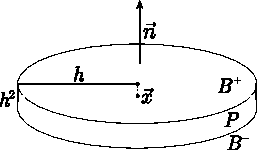
\includegraphics[width=0.6\textwidth]{images/sample.pdf}
%% \caption[caption za v kazalo]{Dolg caption pod sliko}
%  \caption[Primer vektorske slike.]{Primer vektorske slike z oznakami v enaki pisavi, kot jo
%     uporablja \LaTeX{}.  Narejena je s programom Inkscape, \LaTeX{} oznake so importane v
%     Inkscape iz pomožnega PDF.}
%  \label{fig:sample}
%\end{figure}
%
%\begin{figure}[h]
%  \centering
%  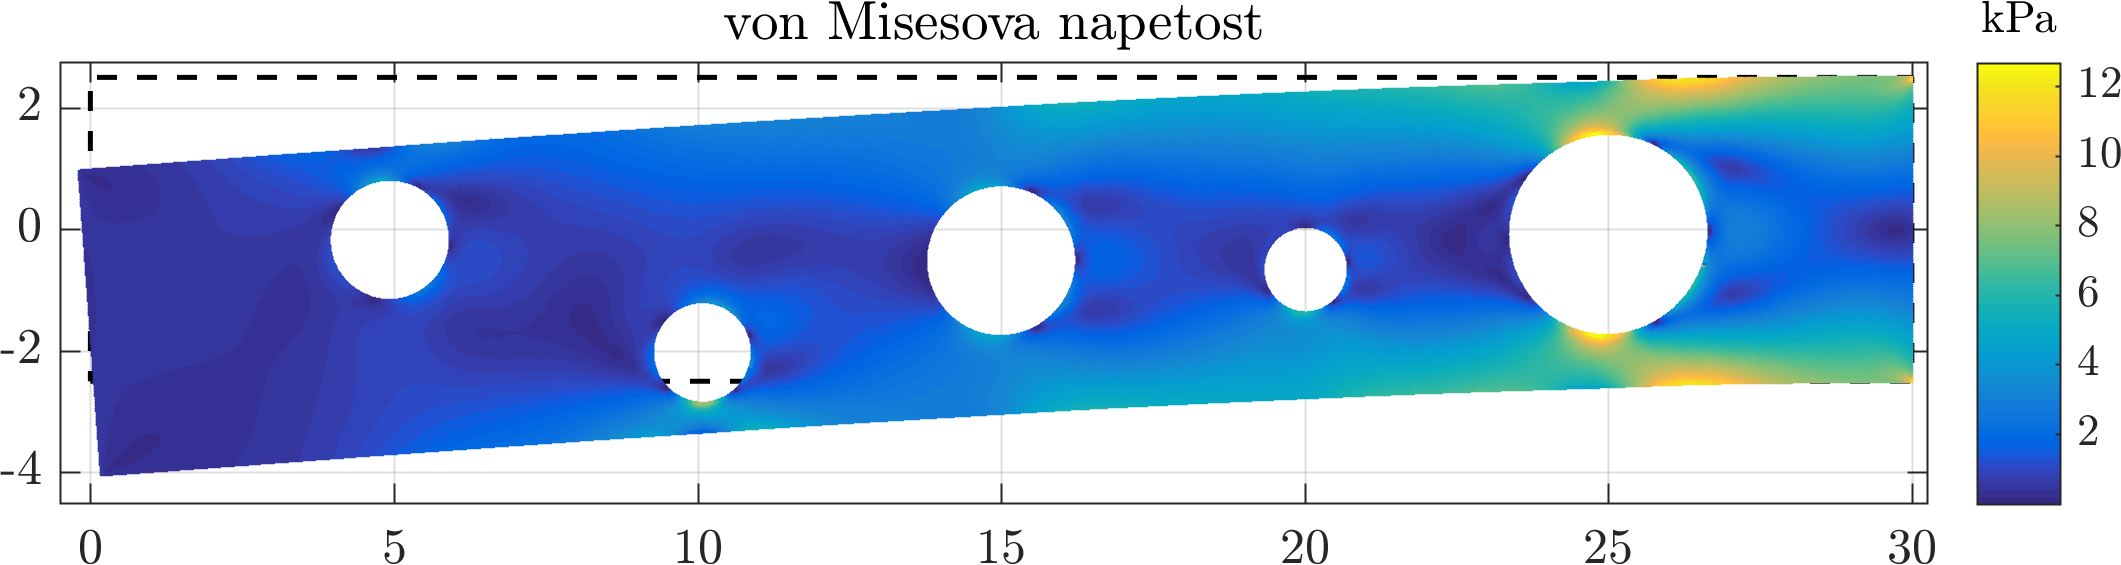
\includegraphics[width=0.8\textwidth]{images/image.png}
%  \caption[Primer bitne slike.]{Primer bitne slike, izvožene iz Matlaba. Poskrbite, da so slike v
%  dovolj visoki resoluciji in da ne vsebujejo prosojnih elementov (to zahteva PDF/A-1b format).}
%  \label{fig:image}
%\end{figure}
%
%\subsection{Kako narediti stvarno kazalo}
%Dodate ukaze \verb|\index{polje}| na besede, kjer je pojavijo, kot tukaj\index{tukaj}.
%Več o stvarnih kazalih je na voljo na \url{https://en.wikibooks.org/wiki/LaTeX/Indexing}.
%
%\subsection{Navajanje literature}
%%Članke citiramo z uporabo \verb|\cite{label}|, \verb|\cite[text]{label}| ali pa več naenkrat s
%%\verb|\cite\{label1, label2}|. Tudi tukaj predhodno besedo in citat povežemo z nedeljivim presledkom
%%$\sim$. Na primer~\cite{chen2006meshless,liu2001point}, ali pa \cite{kibriya2007empirical}, ali pa
%%\cite[str.\ 12]{trobec2015parallel}, \cite[enačba (2.3)]{pereira2016convergence}.
%%Vnosi iz \verb|.bib| datoteke, ki niso citirani, se ne prikažejo v seznamu literature, zato jih
%%tukaj citiram.~\cite{vene2000categorical}, \cite{gregoric2017stopniceni}, \cite{slak2015induktivni},
%%\cite{nsphere}, \cite{kearsley1975linearly}, \cite{STtemplate}, \cite{NunbergerTand}.
%
%Tu na novo citiram \cite{DPHclanek1}, \cite{DPHclanek2}, \cite{beltranmonterde}, \cite{choi2002clifford},
%\cite{struik1961lectures}, \cite{kreyszig2019differential}, \cite{faroukietal2004}, \cite{farouki2008pythagorean}. 

% Literatura:
% Primer navajanja na http://www.fmf.uni-lj.si/storage/24240/LiteraturaM.pdf,
% ampak bi moral stil poskrbeti za vse. Reference se uredijo po abecedi.
% Če nobena izbira izmed @book, @atricle,... ni ok, potem se lahko vse napiše v
% @misc pod note={} in deluje tako kot normalen LaTeX.
% Komentar v bib datoteki se naredi samo s parom { }
% Za urejanje literature avtor priporoča program Jabref, ki zna tudi avtomatsko
% okrajšati imena revij. Za pravilno sortiranje vnosov brez avtorja, uporabite
% polje key={ }, kot v primeru.
% V primeru napak ustvarite issue na GitHubu ali pišite na jure.slak@fmf.uni-lj.si.
\cleardoublepage                           % na desni strani
\phantomsection                            % da prav delujejo hiperlinki
\addcontentsline{toc}{section}{\bibname}   % dodajmo v kazalo
\bibliographystyle{fmf-sl}                 % uporabljen stil je v datoteki fmf-sl.bst, na voljo tudi angleška verzija
\bibliography{literatura.bib}                 % literatura je v datoteki, definirani na začetku
% TeXStudio zmede \ zgoraj, tako da lahko notri napišeš dejansko ime .bib datoteke, če ti
% ne delajo predlogi citatov.

% Za stvarno kazalo
\cleardoublepage                           % na desni strani
\phantomsection                            % da prav delujejo hiperlinki
\addcontentsline{toc}{section}{\indexname} % dodajmo v kazalo
\printindex

\end{document}
